\section{Properties of Estimators}
For an estimator $\hat{\theta}_n$ over available sample of size $n$, we have the following properties.
\begin{itemize}
	\item \textbf{Unbiased}: $\EE[\hat{\theta} - \theta] = 0$.
	\item \textbf{Consistent}: $\displaystyle \lim _{n\to \infty } p{\big (}|\hat{\theta}_{n}-\theta |>\varepsilon {\big )}=0$, or $\hat{\theta}_{n} \overset{p}{\longrightarrow} \theta $.
	\item \textbf{Efficient}: $\hat{\theta}$ achieves equality in CRLB (Sec.~\ref{sec:CRLB}). In other word, $\hat{\theta}$ minimizes $\EE\left[(\hat{\theta} - \theta)^2\right]$.
	\item \textbf{Asymptotically Efficient}: $\hat{\theta}_n$ is efficient as $ n \rightarrow \infty$.
	\item \textbf{Minimum-variance Unbiased Estimator (MVUE)}: An unbiased estimator whose variance is lower than any other unbiased estimator for all possible values of parameter $\hat{\theta}$, i.e., $\mathrm{Var}[\hat{\theta}_{\rm MVUE}] \leq \mathrm{Var}[\hat{\theta}],\ \forall \hat{\theta}$.
\end{itemize}
Towards better understanding of the properties, please note that:
\begin{itemize}
	\item $ \underbrace{\EE\left[\left(\hat{\theta} - \theta\right)^2\right]}_{\mathrm{MSE}(\hat{\theta}, \theta)} = \underbrace{\EE\left[\left(\hat{\theta} - \EE[\theta]\right)^2\right]}_{\mathrm{Var}\left[\hat{\theta}\right]} + \underbrace{\EE\left[\hat{\theta} - \theta\right]^2}_{\text{bias}^2} = \sigma^2 + b^2$. 
	\item $\lim_{n \rightarrow \infty} \mathrm{MSE}\left(\hat{\theta}_n, \theta\right) = 0$ $\Longrightarrow$ Consistency (can be proved by \emph{Chebyshev's} inequality).
	\item Unbiased \& efficient estimator $\Longrightarrow$ minimum-variance, or MVUE.
	\item Unbiased \& minimum-variance $\not\Rightarrow$ efficient estimator (CRLB is not easily achieved). 
\end{itemize}

\begin{property}[Bias after Averaging]
	Assume we have a set of estimators $f_1, \cdots, f_B$. The averaging estimator $\bar{f} = \frac{1}{B} \sum_{i=1}^B f_i$ has the bias as
\begin{equation}
	\mathrm{bias}[\bar{f}(\bfx)] = \E{\bfx, y \sim \cD}{\bar{f}(\bfx) - y} = \frac{1}{B} \sum_{i=1}^B \left(\E{\bfx, y \sim \cD}{{f_i}(\bfx) - y}  \right) =  \frac{1}{B} \sum_{i=1}^B \mathrm{bias}[{f}_i].
\end{equation}
\end{property}
\remark An unbiased estimator remains unbiased after averaging.

\begin{property}[variance after Averaging]
	Assume we have a set of estimators $f_1, \cdots, f_B$. The averaging estimator $\bar{f} = \frac{1}{B} \sum_{i=1}^B f_i$ has the variance as
	\begin{align}
	\mathrm{Var}[\bar{f}(\bfx)] & = \E{\bfx, y \sim \cD}{\left(\bar{f}(\bfx) - \E{\bfx \sim \cD}{\bar{f}(\bfx)}\right)^2} \\
	& =  \E{\bfx, y \sim \cD}{\left(\frac{1}{B} \sum_{i=1}^B \left({f_i}(\bfx) - \E{\bfx \sim \cD}{{f_i}(\bfx)}\right)\right)^2} \\
	& = \frac{1}{B^2} \sum_{i=1}^B \mathrm{Var}[{f_i}(\bfx)] + \frac{1}{B^2} \sum_{i=1}^B \sum_{j=1, j\neq i}^B \mathrm{Cov}[{f_i}(\bfx), {f_j}(\bfx)]
	\end{align} 
\end{property}
\remark If the covariances are neglectable, we can approximate it as $\mathrm{Var}[\bar{f}(\bfx)] \approx \sigma^2 / B $, which means the variance will reduced by a factor of $1/B$.
  
\section{Bayesianism and Frequentism}
\begin{table}[h]
\center
\begin{adjustbox}{width=1\textwidth}
\begin{tabular}{l l l}
		\toprule
		 & \textbf{Bayesian method} & \textbf{Frequentist method} \\
		 \midrule
		 Function & provides a \textbf{predictive distribution} & provides a \textbf{single-point} estimator \\
		 Method & Bayesian inference & Maximum Likelihood Estimator (MLE) \\ \midrule
		 Assumption & a prior distribution $p(\theta)$  & a parametric model $\theta$ \\
		 Likelihood &  conditional distribution $p(y \mid \theta)$ & likelihood function $L(\theta) = \prod_i p(y_i \mid \theta)$ \\
		 Estimator & posterior distribution: & maximum-likelihood estimator:  \\
		 & $\displaystyle p(\theta \mid y) = \frac{p(\theta)\, p(y\mid \theta)}{p(y)}$ & $\hat{\theta}_{MLE} = \argmax_\theta L(\theta)$ \\ \midrule
		 Remarks & priors induce a regularization term & consistency: $\hat{\theta}_{n} \overset{p}{\longrightarrow} \theta $  \\
		 & & asym. normal: $\sqrt{n} (\theta - \hat{\theta}_n) \longrightarrow \mathcal{N}(0, \mathcal{I}(\theta)^{-1}) $ \\
		 & & asym. efficient: achieves CRLB when $n \rightarrow \infty$\\
		\toprule
	\end{tabular}
\end{adjustbox}
\end{table}

Some useful facts of Maximum Likelihood Estimator (MLE): 
\begin{itemize}
	\item An unbiased MLE has the minimum variance as $n \rightarrow \infty$ compared to all other \textbf{unbiased} estimators. \marginpar{\footnotesize Most nice properties of MLE require $n \rightarrow \infty$. 

For a small $n$, MLE may not be a good estimator.}
	\item Biased estimators may have lower variance than MLE as $n \rightarrow \infty$, e.g. the \emph{James-Stein} estimator. 
	\item MLE is \textbf{not} always unbiased, e.g. the MLE for $\theta$ in $\mathrm{Uniform}(0, \theta)$ is $\onehalf \max\{X_i\} < \onehalf \theta $.
	\item MLE of \emph{i.i.d.} observations is always consistent and asymptotically normal.
	\item  If $\hat{\theta}$ is the MLE of $\theta$, for any measurable function $g(\cdot)$, $g(\hat{\theta})$ is also the MLE of $g(\theta)$.
\end{itemize}

\section{Cram\'er-Rao Lower Bound}\label{sec:CRLB}
\begin{definition}[Fisher Information]\label{proof:fisher}
	Given the likelihood $p(x \mid \theta)$ for $\theta \in \Theta $, the Fisher Information $\mathcal{I}(\theta)$ for $\theta$ is 	$$
	\mathcal{I}(\theta) = -\EE_{x\mid \theta}\left[\frac{\partial^{2} \log p(x \mid \theta)}{\partial \theta^{2}}\right] = \EE_{x\mid\theta}\left[\left(\frac{\partial\log p(x \mid \theta)}{\partial \theta}\right)^2 \right]
	$$
\end{definition}
\begin{proof} We need to prove that the values of the expectation are the same. 
For similarity, we introduce the Score Function $\Lambda(\theta)$, which is the deviation of the log likelihood,
\begin{equation}
	\Lambda(x;\theta) = \diff{\theta}\log p(x\mid \theta) = \frac{1}{p(x\mid \theta)}\, \diff{\theta} p(x\mid \theta)
\end{equation}
Obviously, the expectation of $\Lambda(x;\theta)$ is
\begin{align}\label{eq:ex_lambda}
	\EE_{x\mid \theta}[\Lambda(x;\theta)] &= \int p(x\mid \theta) \frac{1}{p(x\mid \theta)}\, \diff{\theta} p(x\mid \theta) \dx \\
	&= \diff{\theta} \int p(x\mid \theta) \dx \\
	&= 0
	\end{align}
According to Eq.~\ref{eq:ex_lambda},
\begin{equation}
	\EE_{x\mid \theta}[\Lambda] = \int p(x\mid \theta) \diff{\theta}\log p(x\mid \theta) = 0
\end{equation}
Differentiate w.r.t. $\theta$ and take the derivative inside gives \footnote{Refer to the slides: \url{https://www.stat.tamu.edu/~suhasini/teaching613/inference.pdf}}
,
\begin{align}
0 &= \int \frac{\partial^{2} \log p(x \mid \theta)}{\partial \theta^{2}} p(x \mid \theta) \dx+\int \frac{\partial \log p(x \mid \theta)}{\partial \theta} \frac{\partial p(x \mid \theta)}{\partial \theta} \dx \\
&= \int \frac{\partial^{2} \log p(x \mid \theta)}{\partial \theta^{2}} p(x \mid \theta) \dx+\int \frac{\partial \log p(x \mid \theta)}{\partial \theta} \frac{1}{p(x \mid \theta)} \frac{\partial p(x \mid \theta)}{\partial \theta} p(x \mid \theta) \dx\\
&= \int \frac{\partial^{2} \log p(x \mid \theta)}{\partial \theta^{2}} p(x \mid \theta) \dx+\int\left(\frac{\partial \log p(x \mid \theta)}{\partial \theta}\right)^{2} p(x \mid \theta) \dx \\
&= \EE_{x\mid\theta}\left[\frac{\partial^{2} \log p(x \mid \theta)}{\partial \theta^{2}}\right] + \EE_{x\mid\theta}\left[\left(\frac{\partial\log p(x \mid \theta)}{\partial \theta}\right)^2\right]
\end{align}
\end{proof}

The Fisher Information can be also written as the variance.
\begin{equation}
	\mathcal{I}(\theta) = \EE_{x\mid\theta}\left[\left(\frac{\partial\log p(x \mid \theta)}{\partial \theta}\right)^2 \right] - \underbrace{\EE_{x\mid\theta}\left[\frac{\partial\log p(x \mid \theta)}{\partial \theta} \right]^2}_{\EE[\Lambda]^2 = 0}
 = \mathbb{V}_{x\mid\theta}\left[\diff{\theta} \log p(x \mid \theta)\right]
\end{equation}
If there are $n$ independent observations, then
\begin{equation}
	\mathcal{I}_n(\theta) = n \, \mathcal{I}(\theta)
\end{equation}

\begin{theorem}[Cram\'er-Rao Lower Bound, CRLB]
	Given the likelihood $p(x \mid \theta)$ for $\theta \in \Theta $, the Fisher Information $\mathcal{I}(\theta)$ for $\theta$, then the expected deviation of a estimator $\hat{\theta}$ with bias $b = \EE_{x\mid \theta}[\hat{\theta} - \theta]$ to the true estimator $\theta$ satisfies
$$
		\EE_{x\mid \theta}[(\hat{\theta} - \theta)^2] \geq \left(\Diff{b}{\theta} + 1\right)^2 \mathcal{I}^{-1}(\theta) + b^2, \where \mathcal{I}(\theta) = -\EE_{x\mid \theta}\left[\ddiff{\theta} \log p(x\mid \theta)\right]
$$
\end{theorem}
\begin{proof} 
We follow the same notation in the Proof.~\ref{proof:fisher}.
The expectation of $\Lambda \hat{\theta}$ is
\begin{align}
	\EE_{x\mid \theta}[\Lambda(x;\theta)\ \hat{\theta}(x)] &= \int p(x\mid \theta) \frac{1}{p(x\mid \theta)}\, \diff{\theta} p(x\mid \theta)\, \hat{\theta}(x) \dx \\
	&= \int \hat{\theta}(x) \diff{\theta} p(x\mid \theta) \dx \\
	&= \diff{\theta} \int \hat{\theta}(x) p(x\mid \theta) \dx \\
	&= \diff{\theta} \EE_{x\mid\theta}[\hat{\theta}(x)] \\
	&= \diff{\theta} \EE_{x\mid\theta}[\hat{\theta}(x) - \theta] + 1
	\end{align}
Recalling that the \textit{Cauchy-Schwartz} inequality that $\EE[XY]^2 \leq \EE[X^2]\ \EE[Y^2] $, we have
\begin{align}
	\EE_{x\mid \theta}[\Lambda(x;\theta)\ \hat{\theta}(x)]^2 &= \EE_{x\mid \theta}\left[(\Lambda - \EE_{x\mid \theta}[\Lambda]) \, (\hat{\theta} - \EE_{x\mid \theta}[\hat{\theta}])\right]^2 \\
	&\leq  \EE_{x\mid \theta}\left[(\Lambda - \EE_{x\mid \theta}[\Lambda])^2\right] \, \EE_{x\mid \theta}\left[(\hat{\theta} - \EE_{x\mid \theta}[\hat{\theta}])^2\right] \\
	&=\EE_{x\mid \theta}[\Lambda^2]\, \EE_{x\mid \theta}\left[(\hat{\theta} - \EE_{x\mid \theta}[\hat{\theta}])^2\right]
\end{align}
Therefore, 
\begin{align}
	\EE_{x\mid \theta}\left[(\hat{\theta} - \EE_{x\mid \theta}[\hat{\theta}])^2\right] &\geq \frac{\EE_{x\mid \theta}[\Lambda\ \hat{\theta}]^2}{\EE_{x\mid \theta}[\Lambda^2]} \\
	\EE_{x\mid \theta}[\hat{\theta}^2] - \EE_{x\mid \theta}[\hat{\theta}]^2 & \geq \frac{\left(\diff{\theta} \EE_{x\mid\theta}[\hat{\theta}(x) - \theta] + 1\right)^2}{\mathcal{I}(\theta)} \\
	\EE_{x\mid \theta}[(\hat{\theta}-\theta)^2] - \EE[\hat{\theta} - \theta]^2 & \geq \frac{\left(\diff{\theta} \EE_{x\mid\theta}[\hat{\theta}(x) - \theta] + 1\right)^2}{\mathcal{I}(\theta)} \\
	\EE_{x\mid \theta}[(\hat{\theta}-\theta)^2] & \geq \frac{\left(\Diff{b}{\theta} + 1\right)^2}{\mathcal{I}(\theta)}	+ b^2
\end{align}
\end{proof}

The condition that a estimator $\hat{\theta}$ attains the CRLB is
\begin{equation}
	\hat{\theta} = \alpha + \beta\cdot  \frac{\partial\log p(x \mid \theta)}{\partial \theta}, \quad \alpha, \beta \in \R
\end{equation}
The maximum likelihood estimator $\hat{\theta}_{MLE}$ is asymptotically efficient, i.e.,
\begin{equation}
	\lim_{n\rightarrow \infty} \EE_{x\mid \theta}[(\hat{\theta}_{MLE}-\theta)^2] = \frac{1}{n\, \mathcal{I}(\theta)}
\end{equation}
%
%\section{Hilbert Space}
%\begin{figure}[htbp]
%\center
%	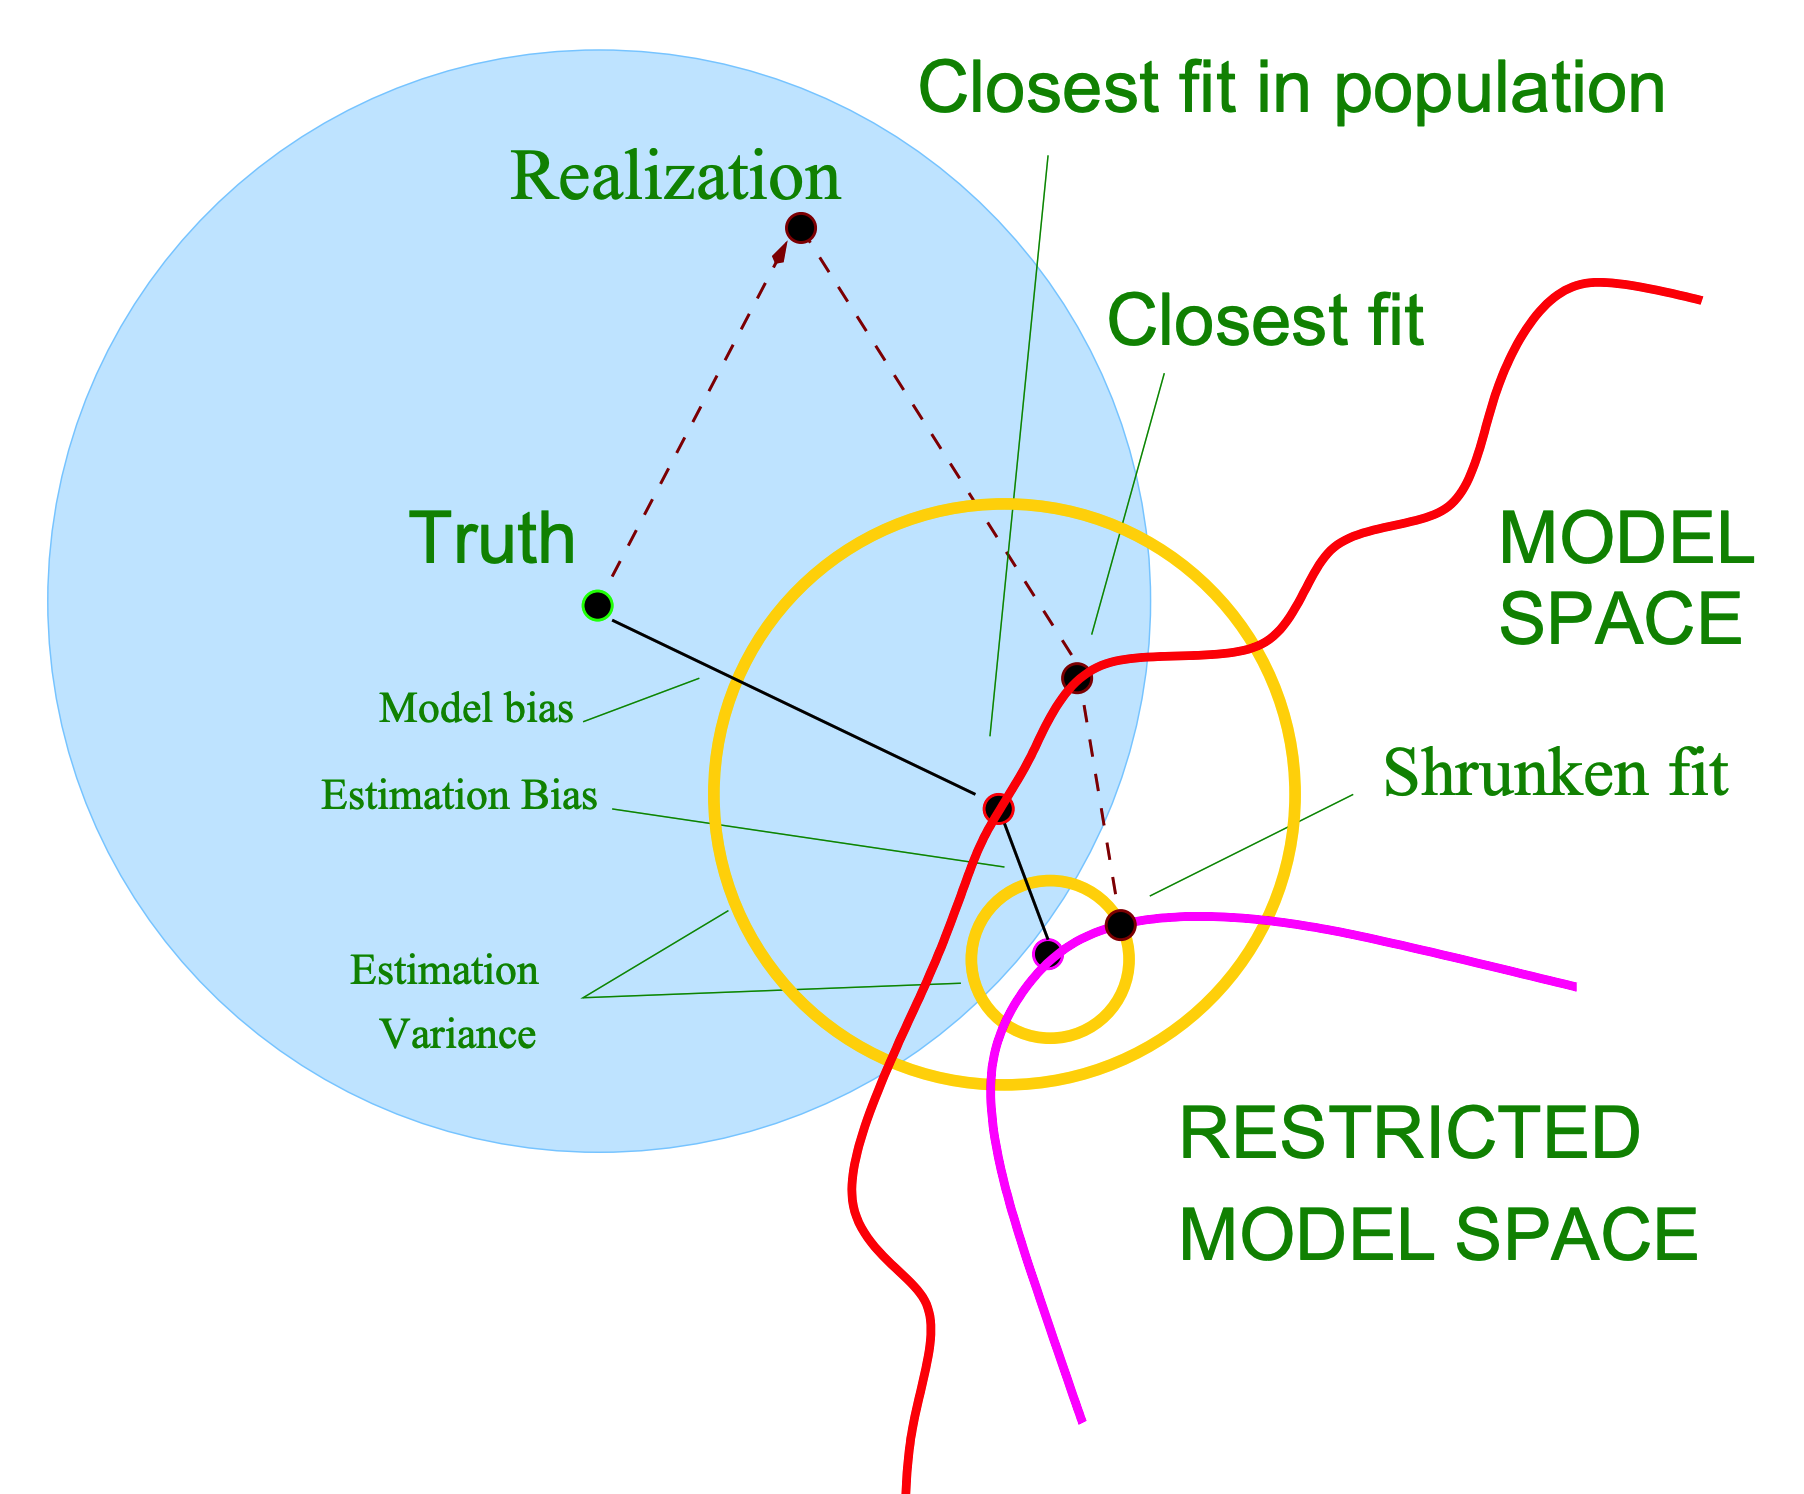
\includegraphics[width=0.8\textwidth]{figures/bias_variance}
%\end{figure}